\documentclass[11pt]{article}
\usepackage[a4paper,margin=2cm]{geometry}
\usepackage{amsmath}
\usepackage{enumitem}
\usepackage{booktabs}
\usepackage{array}
\usepackage{graphicx}
\usepackage{xcolor}
\usepackage{parskip}
\setlist{itemsep=3pt, topsep=3pt}
\renewcommand{\arraystretch}{1.3}
\newcommand{\menu}[1]{\textbf{#1}}

\begin{document}

{\LARGE\bfseries Raspberry Pi as the MQTT gateway}\\[4pt]
{\large NodeMCU publisher $\rightarrow$ Pi broker $\rightarrow$ laptop subscriber, plus packet capture on the Pi}

\vspace{6pt}
This is step 1 and 2 of the TinyIDS experiment. In TinyIDS the Raspberry Pi is the \textbf{gateway}: all sensor traffic must flow \emph{into} the Pi,
because that is where the \textbf{IDS (Intrusion Detection System)} will watch the packets. So the \textbf{MQTT (Message Queuing Telemetry Transport)} broker runs on the Pi.

\section*{The setup}
\begin{center}
\texttt{NodeMCU (publisher)}\\
$\downarrow$ {\small Wi-Fi, MQTT, topic \texttt{test/01}}\\
\texttt{Raspberry Pi (Mosquitto broker = gateway)}\\
$\downarrow$ {\small MQTT}\\
\texttt{Windows laptop (sub.py)}
\end{center}

\begin{tabular}{@{}l l l@{}}
\toprule
\textbf{Device} & \textbf{Role} & \textbf{IP (college Wi-Fi, 06 Nov 2026)} \\
\midrule
NodeMCU (ESP8266) & publisher, topic \texttt{test/01} & 172.29.1.103 \\
Raspberry Pi 4 & broker (Mosquitto) = gateway & 172.29.1.135 \\
Windows laptop & subscriber (\texttt{sub.py}) & 172.29.1.102 \\
\bottomrule
\end{tabular}

All three are on the college Wi-Fi (IIITA). The IPs are given out automatically (DHCP = Dynamic Host Configuration Protocol) and
\textbf{change from day to day}; on a phone hotspot they usually stay the same. Find the Pi's current IP with \texttt{hostname -I} on the Pi.

\textbf{Files used} (from the \texttt{mqtt\_test} folder; no new code was needed):
\begin{itemize}
\item \texttt{nodemcu\_mqtt\_pub/nodemcu\_mqtt\_pub.ino} on the NodeMCU
\item \texttt{sub.py} on the laptop
\end{itemize}

\section*{Step 1: Check the Pi's broker}
The lab Pi already has Mosquitto installed and configured. Connect to the Pi (monitor + keyboard, or SSH = Secure Shell: \texttt{ssh pi@<pi-ip>}) and check:
\begin{verbatim}
sudo systemctl status mosquitto            # should say: active (running)
cat /etc/mosquitto/conf.d/local.conf
\end{verbatim}
\texttt{local.conf} contains:
\begin{verbatim}
listener 1883
allow_anonymous true
\end{verbatim}
\begin{itemize}
\item \texttt{listener 1883} = accept connections from \emph{other} devices on port 1883 (not only from the Pi itself).
\item \texttt{allow\_anonymous true} = no username/password needed (fine for a lab test).
\end{itemize}
\textbf{Don't add a second config file with another \texttt{listener 1883}}: two listeners on the same port stop Mosquitto from starting.

\textit{Fresh Pi without Mosquitto?} \texttt{sudo apt install -y mosquitto mosquitto-clients}, then create \texttt{local.conf} with the two lines above and
\texttt{sudo systemctl restart mosquitto}. (Needs the proxy on the college network: see Step 5.)

%% -------------------------------------------------------------------
\newpage
\section*{Step 2: Point the NodeMCU at the Pi}
In \texttt{nodemcu\_mqtt\_pub.ino}, keep exactly one \texttt{BROKER} line uncommented and set it to the Pi's IP:
\begin{verbatim}
//const char* BROKER = "172.29.0.43";       // laptop broker (not used now)
const char* BROKER = "172.29.1.135";        // the Pi
// const char* BROKER = "broker.hivemq.com"; // public broker (hotspot only)
\end{verbatim}
Upload, then check the Serial Monitor (9600 baud): \texttt{Connecting to MQTT broker 172.29.1.135 ... OK} followed by \texttt{sent \{...\}} every 2 seconds.

\section*{Step 3: Receive on the Pi}
On the Pi:
\begin{verbatim}
mosquitto_sub -h localhost -t test/01 -v
\end{verbatim}
\texttt{-h localhost} = the broker on this Pi, \texttt{-t test/01} = the topic, \texttt{-v} = also print the topic name. Output every 2 seconds:
\begin{verbatim}
test/01 {"uptime_s":733,"rssi_dbm":-76,"free_heap":50112,"a0":5}
test/01 {"uptime_s":735,"rssi_dbm":-76,"free_heap":50112,"a0":4}
\end{verbatim}
Stop with Ctrl+C.

\section*{Step 4: Receive on the Windows laptop}
\texttt{sub.py} takes the broker's address as an argument (no need to edit the file):
\begin{verbatim}
cd C:\Users\HOME\Documents\iot\project_final\mqtt_test
python sub.py 172.29.1.135
\end{verbatim}
\begin{verbatim}
Connected to 172.29.1.135, listening on 'test/01' ...
18:58:40  test/01  {"uptime_s":127,"rssi_dbm":-75,"free_heap":50112,"a0":4}
18:58:42  test/01  {"uptime_s":129,"rssi_dbm":-76,"free_heap":50112,"a0":5}
\end{verbatim}
\texttt{python sub.py} with no argument uses \texttt{localhost} (a broker on the laptop itself).

\textbf{Result:} the same message reaches both the Pi and the laptop. The broker on the Pi forwards every message to everyone subscribed to \texttt{test/01}.

%% -------------------------------------------------------------------
\newpage
\section*{Step 5: Internet on the Pi through the college proxy (for installing software)}
On the college network, the Pi can only reach the internet through the proxy (host \texttt{172.31.2.3}, port \texttt{8080}, no username/password).
Without it, \texttt{apt} fails with \texttt{403 Forbidden}.

\textbf{Turn the proxy ON for apt} (the Debian/Raspberry Pi package installer):
\begin{verbatim}
echo 'Acquire::http::Proxy "http://172.31.2.3:8080";
Acquire::https::Proxy "http://172.31.2.3:8080";' \
  | sudo tee /etc/apt/apt.conf.d/95proxy
\end{verbatim}
This creates one small file. Test: \texttt{sudo apt update} or \texttt{sudo apt install tcpdump}.

\textbf{Turn it OFF / delete it} (e.g.\ when the Pi is on a phone hotspot, where the proxy does not exist):
\begin{verbatim}
sudo rm /etc/apt/apt.conf.d/95proxy
\end{verbatim}
\textbf{Check} whether it is on: \texttt{cat /etc/apt/apt.conf.d/95proxy} (``No such file'' = off).

For a single command that needs the internet (e.g.\ \texttt{curl}), you can pass the proxy just for that command with \texttt{-x http://172.31.2.3:8080}.
Nothing is saved, so there is nothing to undo.

\section*{Step 6: Fix the Pi's clock}
\textbf{Problem:} the Pi thought it was still the previous day. \texttt{apt} complained
\texttt{Verifying signature: Not live until 2026-11-06T10:17:25Z}. The Pi has no battery-backed clock and normally sets its time from the internet
using \textbf{NTP (Network Time Protocol)}; the college network blocks NTP, so the clock goes wrong. Wrong time = wrong timestamps in logs and alerts,
which matter for the report.

\textbf{Fix:} read the current time from Google's web server (through the proxy) and set the clock to it:
\begin{verbatim}
sudo date -s "$(curl -sI -x http://172.31.2.3:8080 https://www.google.com \
  | grep -i '^date:' | cut -d' ' -f2-)"
date
\end{verbatim}
How it works: \texttt{curl -sI} asks Google only for the response \emph{headers}; one header is \texttt{date: Fri, 06 Nov 2026 13:38:55 GMT};
\texttt{grep}/\texttt{cut} keep just the date part; \texttt{date -s} sets the Pi's clock to it. Result:
\begin{verbatim}
Friday 06 November 2026 07:08:55 PM IST
\end{verbatim}

\textbf{How to revert / undo:}
\begin{itemize}
\item Nothing permanent was changed: the clock goes back to automatic behaviour on the next reboot.
\item To hand control back to automatic time sync right away: \texttt{sudo timedatectl set-ntp true}
\item Check the time-sync status: \texttt{timedatectl} (look at ``System clock synchronized'').
\item On a phone hotspot NTP works, so the clock fixes itself; on college Wi-Fi run the fix again after each reboot.
\end{itemize}

%% -------------------------------------------------------------------
\newpage
\section*{Step 7: Capture the traffic on the Pi (base of the IDS)}
The IDS will work by capturing packets on the Pi. \textbf{tcpdump} is a command-line packet capture tool (like Wireshark without the window):
\begin{verbatim}
sudo tcpdump -i wlan0 -n port 1883 -c 20
\end{verbatim}
\texttt{-i wlan0} = listen on the Pi's Wi-Fi; \texttt{-n} = show IPs, not names; \texttt{port 1883} = only MQTT traffic; \texttt{-c 20} = stop after 20 packets.

\textbf{Output} (part):
{\small
\begin{verbatim}
19:09:18.630465 IP 172.29.1.103.62463 > 172.29.1.135.1883: Flags [P.], ... length 67
19:09:18.630490 IP 172.29.1.135.1883 > 172.29.1.103.62463: Flags [.], ack 67, ... length 0
19:09:18.630593 IP 172.29.1.135.1883 > 172.29.1.102.57558: Flags [P.], ... length 67
19:09:18.936755 IP 172.29.1.102.57558 > 172.29.1.135.1883: Flags [.], ack 67, ... length 0
...
19:09:25.170392 IP 172.29.1.103.62463 > 172.29.1.135.1883: Flags [P.], ... length 2
19:09:25.170660 IP 172.29.1.135.1883 > 172.29.1.103.62463: Flags [P.], ... length 2
20 packets captured
\end{verbatim}
}

\textbf{How to read it} (every 2 seconds the same pattern of 4 packets):

\noindent\begin{tabular}{@{}>{\raggedright}p{4.8cm} >{\raggedright\arraybackslash}p{11.2cm}@{}}
\toprule
\textbf{Line} & \textbf{Meaning} \\
\midrule
\texttt{.103 > .135 [P.] len 67} & NodeMCU sends one MQTT \textbf{PUBLISH} (67 bytes = the JSON message) to the Pi. \\
\texttt{.135 > .103 [.] len 0} & Pi's TCP \textbf{ACK}: ``got it'' (no data). \\
\texttt{.135 > .102 [P.] len 67} & Pi \textbf{forwards} the same 67-byte message to the laptop (subscriber). \\
\texttt{.102 > .135 [.] len 0} & Laptop's ACK. \\
\texttt{len 2} packets & MQTT \textbf{PINGREQ / PINGRESP}: a tiny ``are you still there?'' keep-alive between NodeMCU and Pi. \\
\bottomrule
\end{tabular}

\begin{itemize}
\item \texttt{Flags [P.]} = \textbf{PSH + ACK} (TCP flags ``push data now'' + ``acknowledge''); \texttt{Flags [.]} = ACK only.
These are exactly the flag columns of the CICIoT2023 dataset (\texttt{psh\_flag\_number}, \texttt{ack\_flag\_number}). This is the bridge between the dataset
and the live traffic: the live IDS will compute the same kind of features from these packets.
\item \texttt{62463}, \texttt{57558} = random ``source ports'' the NodeMCU and laptop picked for their connection; \texttt{1883} = MQTT port.
\item \texttt{0 packets dropped by kernel} = the Pi kept up with the traffic.
\end{itemize}

%% -------------------------------------------------------------------
\section*{Troubleshooting}
\begin{tabular}{@{}>{\raggedright}p{5.6cm} >{\raggedright\arraybackslash}p{10.6cm}@{}}
\toprule
\textbf{Symptom} & \textbf{Fix} \\
\midrule
NodeMCU: \texttt{failed (state -2)} & Wrong Pi IP (check \texttt{hostname -I} on the Pi), or Mosquitto not running (\texttt{sudo systemctl restart mosquitto}). \\
\texttt{sub.py}: connection refused / timeout & Same as above; also check the laptop is on the same Wi-Fi. \\
\texttt{apt}: \texttt{403 Forbidden} & Proxy not set for apt (Step 5). \\
\texttt{apt}: \texttt{Not live until \dots} & Pi clock is wrong (Step 6). \\
\texttt{tcpdump}: command not found & \texttt{sudo apt install tcpdump} (with the proxy on). \\
\bottomrule
\end{tabular}

%% -------------------------------------------------------------------
\newpage
\section*{Result (tested, 06 November 2026)}
NodeMCU sketch with \texttt{BROKER = "172.29.1.135"} (the Pi) and its Serial Monitor showing each message sent:

\vspace{4pt}
\begin{center}
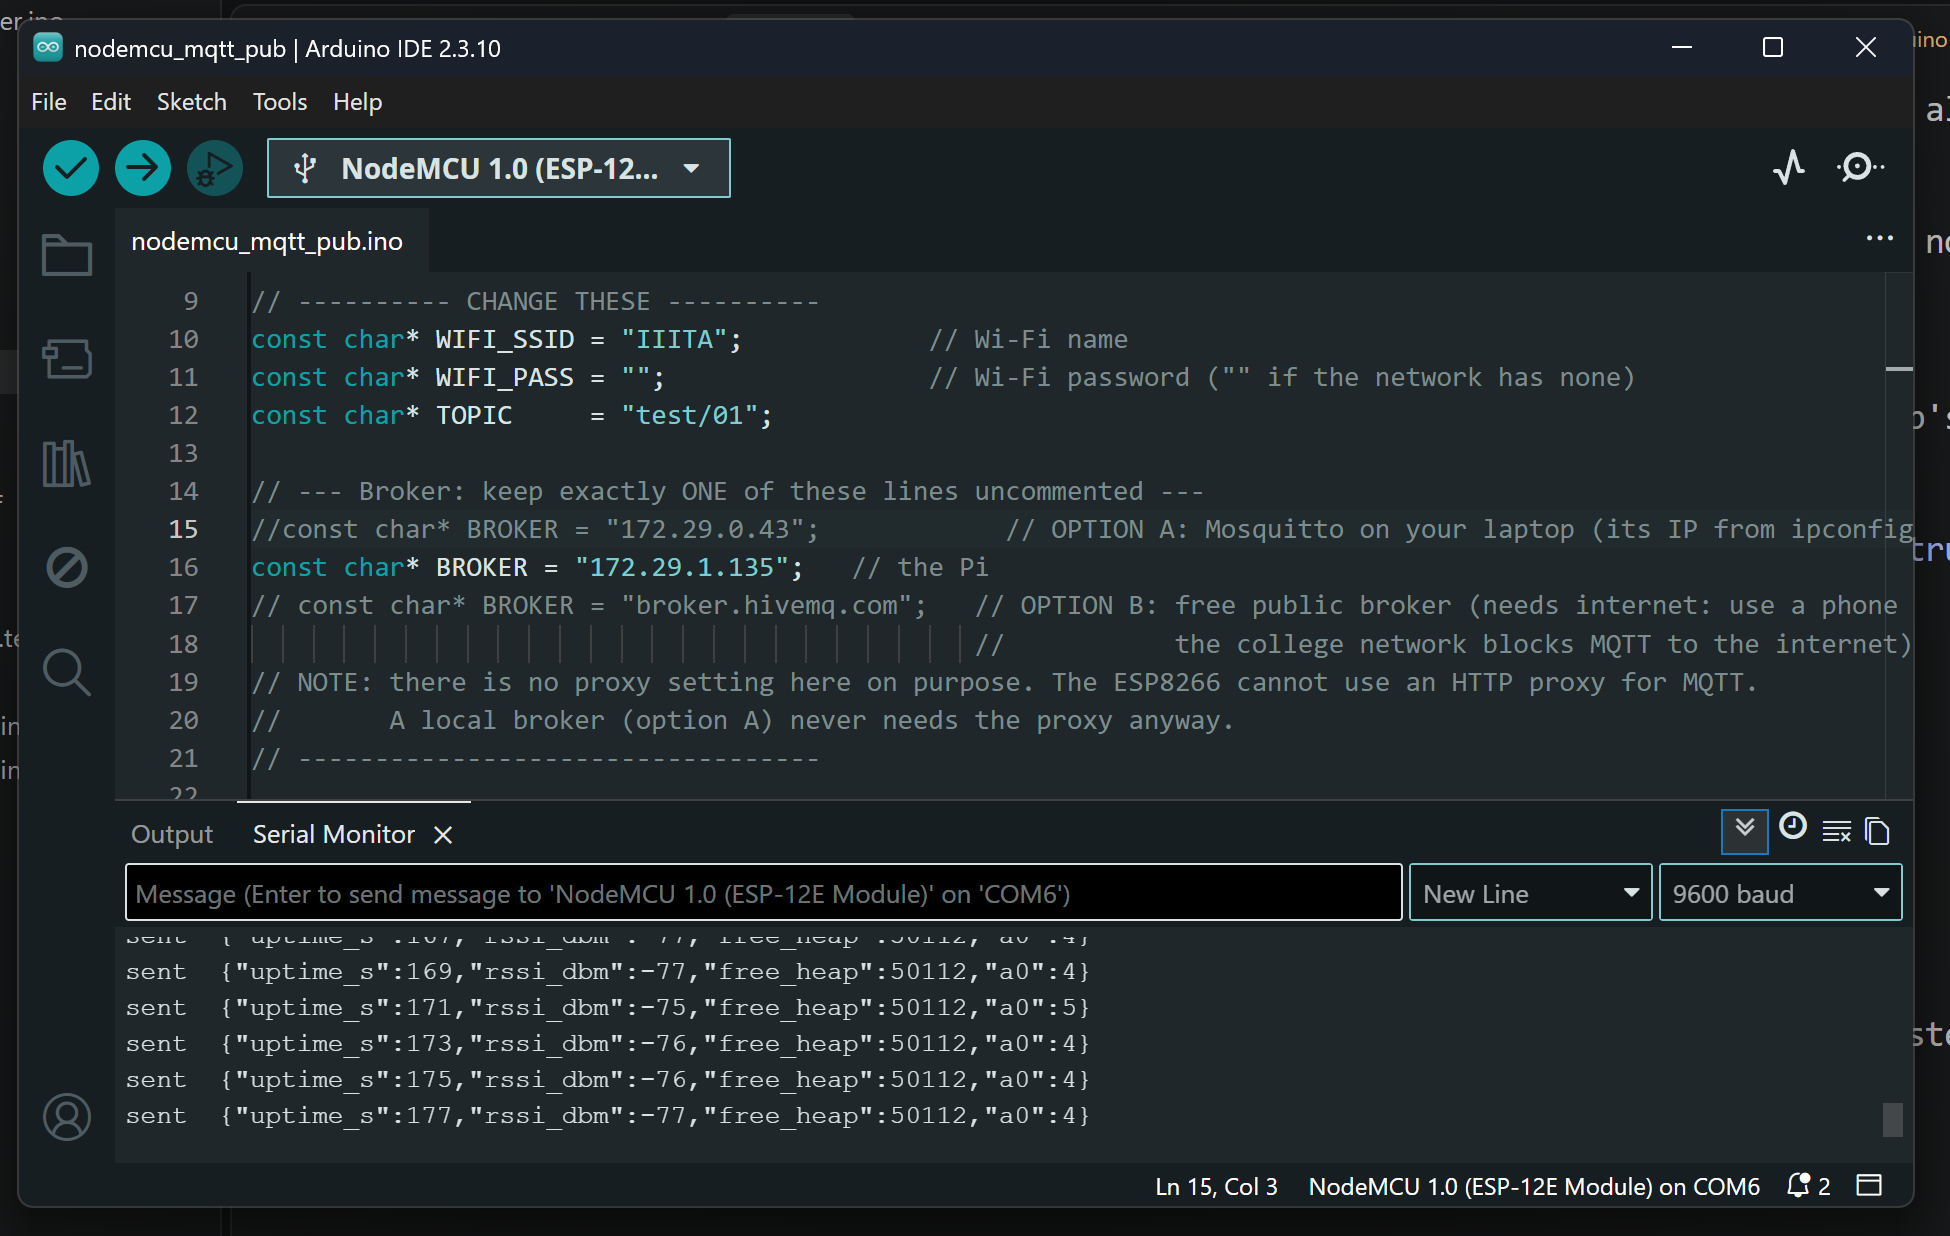
\includegraphics[width=0.95\textwidth]{img/pi_gateway_nodemcu.png}
\end{center}

\vspace{4pt}
At the same time the messages arrived on the Pi (\texttt{mosquitto\_sub}, Step 3), on the laptop (\texttt{python sub.py 172.29.1.135}, Step 4),
and the packets were visible in \texttt{tcpdump} on the Pi (Step 7).

\end{document}
